\documentclass[12pt]{article}
\usepackage{amsmath}
\usepackage{geometry}
\usepackage{tikz}

\geometry{margin=1in}

\begin{document}
\section*{Trigonometric Survival Sheet}

\subsection*{Pythagorean Theorem}
\[
a^2 + b^2 = c^2
\]

\subsection*{Unit Circle Key Values}
\[
\begin{array}{c|c|c|c}
\theta & \sin \theta & \cos \theta & \tan \theta \\
\hline
0 & 0 & 1 & 0 \\
\frac{\pi}{6} & \frac{1}{2} & \frac{\sqrt{3}}{2} & \frac{1}{\sqrt{3}} \\
\frac{\pi}{4} & \frac{\sqrt{2}}{2} & \frac{\sqrt{2}}{2} & 1 \\
\frac{\pi}{3} & \frac{\sqrt{3}}{2} & \frac{1}{2} & \sqrt{3} \\
\frac{\pi}{2} & 1 & 0 & \text{undefined}
\end{array}
\]

\subsection*{Radians and Degrees}
\[
180^\circ = \pi \text{ radians}
\]
\[
\text{degrees} \cdot \frac{\pi}{180}, \quad \text{radians} \cdot \frac{180}{\pi}
\]

\subsection*{Signs by Quadrant}
\[
\text{QI: All}, \quad \text{QII: Sine}, \quad \text{QIII: Tangent}, \quad \text{QIV: Cosine}
\]

\subsection*{Reciprocal Identities}
\[
\sin \theta = \frac{1}{\csc \theta}, \quad 
\cos \theta = \frac{1}{\sec \theta}, \quad 
\tan \theta = \frac{1}{\cot \theta}
\]
\[
\csc \theta = \frac{1}{\sin \theta}, \quad 
\sec \theta = \frac{1}{\cos \theta}, \quad 
\cot \theta = \frac{1}{\tan \theta}
\]

\subsection*{Pythagorean Identities}
\[
\sin^2 \theta + \cos^2 \theta = 1
\]
\[
1 + \tan^2 \theta = \sec^2 \theta
\]
\[
1 + \cot^2 \theta = \csc^2 \theta
\]

\subsection*{Quotient Identities}
\[
\tan \theta = \frac{\sin \theta}{\cos \theta}, 
\quad \cot \theta = \frac{\cos \theta}{\sin \theta}
\]

\subsection*{Cofunction Identities}
\[
\sin \left( \frac{\pi}{2} - \theta \right) = \cos \theta, 
\quad \cos \left( \frac{\pi}{2} - \theta \right) = \sin \theta
\]
\[
\tan \left( \frac{\pi}{2} - \theta \right) = \cot \theta, 
\quad \cot \left( \frac{\pi}{2} - \theta \right) = \tan \theta
\]
\[
\sec \left( \frac{\pi}{2} - \theta \right) = \csc \theta, 
\quad \csc \left( \frac{\pi}{2} - \theta \right) = \sec \theta
\]

\subsection*{Even-Odd Identities}
\[
\sin(-\theta) = -\sin \theta, \quad \cos(-\theta) = \cos \theta
\]
\[
\tan(-\theta) = -\tan \theta, \quad \cot(-\theta) = -\cot \theta
\]
\[
\sec(-\theta) = \sec \theta, \quad \csc(-\theta) = -\csc \theta
\]

\subsection*{Sum and Difference Formulas}
\[
\sin(A \pm B) = \sin A \cos B \pm \cos A \sin B
\]
\[
\cos(A \pm B) = \cos A \cos B \mp \sin A \sin B
\]
\[
\tan(A \pm B) = \frac{\tan A \pm \tan B}{1 \mp \tan A \tan B}
\]

\subsection*{Double Angle Formulas}
\[
\sin(2\theta) = 2 \sin \theta \cos \theta
\]
\[
\cos(2\theta) = \cos^2 \theta - \sin^2 \theta = 2\cos^2 \theta - 1 = 1 - 2\sin^2 \theta
\]
\[
\tan(2\theta) = \frac{2\tan \theta}{1 - \tan^2 \theta}
\]

\subsection*{Half Angle Formulas}
\[
\sin^2 \theta = \frac{1 - \cos(2\theta)}{2}, 
\quad 
\cos^2 \theta = \frac{1 + \cos(2\theta)}{2}
\]
\[
\tan^2 \theta = \frac{1 - \cos(2\theta)}{1 + \cos(2\theta)}, \quad
\tan \theta = \pm \sqrt{\frac{1 - \cos(2\theta)}{1 + \cos(2\theta)}}
\]

\subsection*{Product-to-Sum Formulas}
\[
\sin A \sin B = \tfrac{1}{2}[\cos(A-B) - \cos(A+B)]
\]
\[
\cos A \cos B = \tfrac{1}{2}[\cos(A-B) + \cos(A+B)]
\]
\[
\sin A \cos B = \tfrac{1}{2}[\sin(A+B) + \sin(A-B)]
\]

\subsection*{Sum-to-Product Formulas}
\[
\sin A + \sin B = 2 \sin \left(\tfrac{A+B}{2}\right) \cos \left(\tfrac{A-B}{2}\right)
\]
\[
\sin A - \sin B = 2 \cos \left(\tfrac{A+B}{2}\right) \sin \left(\tfrac{A-B}{2}\right)
\]
\[
\cos A + \cos B = 2 \cos \left(\tfrac{A+B}{2}\right) \cos \left(\tfrac{A-B}{2}\right)
\]
\[
\cos A - \cos B = -2 \sin \left(\tfrac{A+B}{2}\right) \sin \left(\tfrac{A-B}{2}\right)
\]

\subsection*{Inverse Trigonometric Functions}
\[
\sin^{-1}(x), \quad \cos^{-1}(x), \quad \tan^{-1}(x)
\]
\[
\sin^{-1}(x): \left[-\tfrac{\pi}{2}, \tfrac{\pi}{2}\right], \quad
\cos^{-1}(x): [0,\pi], \quad
\tan^{-1}(x): \left(-\tfrac{\pi}{2}, \tfrac{\pi}{2}\right)
\]

\subsection*{Graphing Trig Functions}

\textbf{General Forms:}
\[
y = A \sin(Bx - C) + D, \quad y = A \cos(Bx - C) + D, \quad y = A \tan(Bx - C) + D
\]

\textbf{Parameters:}
\begin{itemize}
    \item Amplitude: $|A|$ (height from midline)
    \item Period: 
    \[
    \text{Sine/Cosine: } \frac{2\pi}{B}, \quad 
    \text{Tangent: } \frac{\pi}{B}
    \]
    \item Phase Shift: $\frac{C}{B}$ (horizontal shift)
    \item Vertical Shift: $D$ (moves graph up/down)
\end{itemize}

\textbf{Example Key Points:}
\[
\begin{array}{c|c|c}
\text{Function} & \text{Period} & \text{Amplitude} \\
\hline
y = 3\sin(2x) & \pi & 3 \\
y = 2\cos\left(x - \frac{\pi}{4}\right) & 2\pi & 2 \\
y = \tan(x) & \pi & \text{undefined}
\end{array}
\]

\subsection*{Trig Function Sketches} %AUTHOR and credit for tikz code
%%%%%  M. S. Rosyidi %%%%%

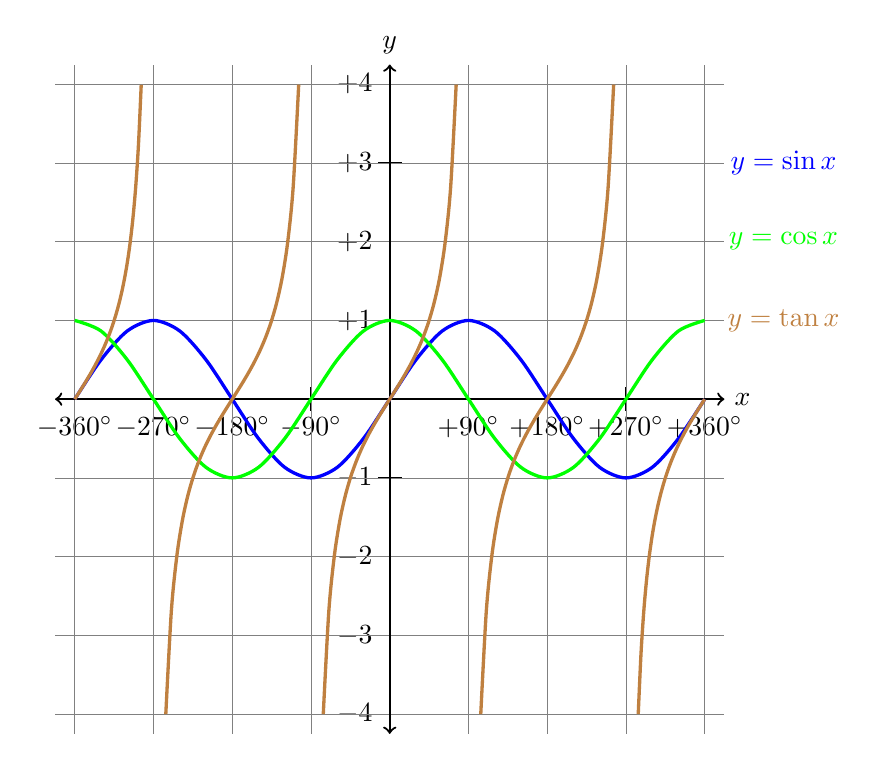
\begin{tikzpicture}[help lines/.style={black!50,very thin}]
	\foreach \x in {-360,-270,-180,-90,+90,+180,+270,+360} \draw ({\x/90},-0.15) -- ({\x/90},+0.15) node[below=7] {$\x^\circ$};
	\foreach \y in {-4,-3,-2,-1,+1,+2,+3,+4} \draw (-0.15,\y) -- (+0.15,\y) node[left=7] {$\y$};
	\draw[help lines] (-4.25,-4.25) grid (4.25,4.25);
	\draw[<->,thick] (-4.25,0)--(4.25,0) node[right] {$x$};
	\draw[<->,thick] (0,-4.25)--(0,4.25) node[above] {$y$};
	\draw[very thick,color=blue ] plot [domain={-360/90}:{360/90},smooth] (\x,{sin(90*\x)});
	\draw[very thick,color=green] plot [domain={-360/90}:{360/90},smooth] (\x,{cos(90*\x)});
	\foreach \i in {0,...,4} \draw[very thick,color=brown] plot [domain={(180*(\i-2)-atan(4)*ceil(\i/4))/90}:{(180*(\i-2)+atan(4)*ceil((4-\i)/4))/90},smooth] (\x,{tan(90*\x)});
	\node[blue ] at (5,3) {$y = \sin x$};
	\node[green] at (5,2) {$y = \cos x$};
	\node[brown] at (5,1) {$y = \tan x$};
\end{tikzpicture}

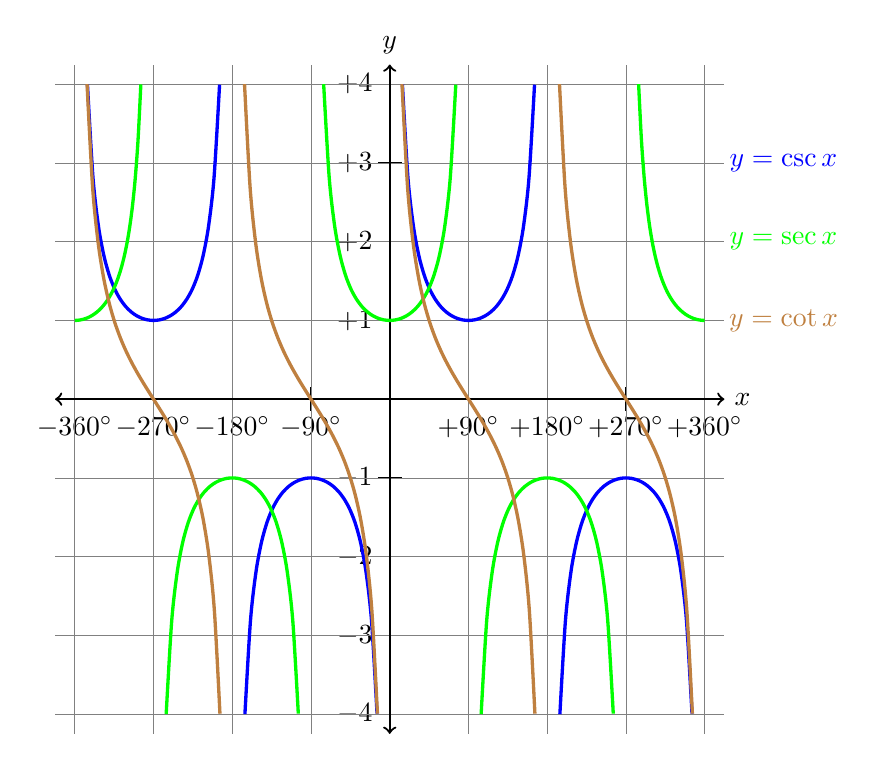
\begin{tikzpicture}[help lines/.style={black!50,very thin}]
	\foreach \x in {-360,-270,-180,-90,+90,+180,+270,+360} \draw ({\x/90},-0.15) -- ({\x/90},+0.15) node[below=7] {$\x^\circ$};
	\foreach \y in {-4,-3,-2,-1,+1,+2,+3,+4} \draw (-0.15,\y) -- (+0.15,\y) node[left=7] {$\y$};
	\draw[help lines] (-4.25,-4.25) grid (4.25,4.25);
	\draw[<->,thick] (-4.25,0)--(4.25,0) node[right] {$x$};
	\draw[<->,thick] (0,-4.25)--(0,4.25) node[above] {$y$};
	\foreach \i in {0,...,3} \draw[very thick,color=blue ] plot [domain={(180*(\i-2)+asin(1/4))/90}:{(180*(\i-1)-asin(1/4))/90},smooth] (\x,{cosec(90*\x)});
	\foreach \i in {0,...,4} \draw[very thick,color=green] plot [domain={(180*(\i-2)-acos(1/4)*ceil(\i/4))/90}:{(180*(\i-2)+acos(1/4)*ceil((4-\i)/4))/90},smooth] (\x,{sec(90*\x)});
	\foreach \i in {0,...,3} \draw[very thick,color=brown] plot [domain={(180*(\i-2)+atan(1/4))/90}:{(180*(\i-1)-atan(1/4))/90},smooth] (\x,{cot(90*\x)});
	\node[blue ] at (5,3) {$y = \csc x$};
	\node[green] at (5,2) {$y = \sec x$};
	\node[brown] at (5,1) {$y = \cot x$};
\end{tikzpicture}

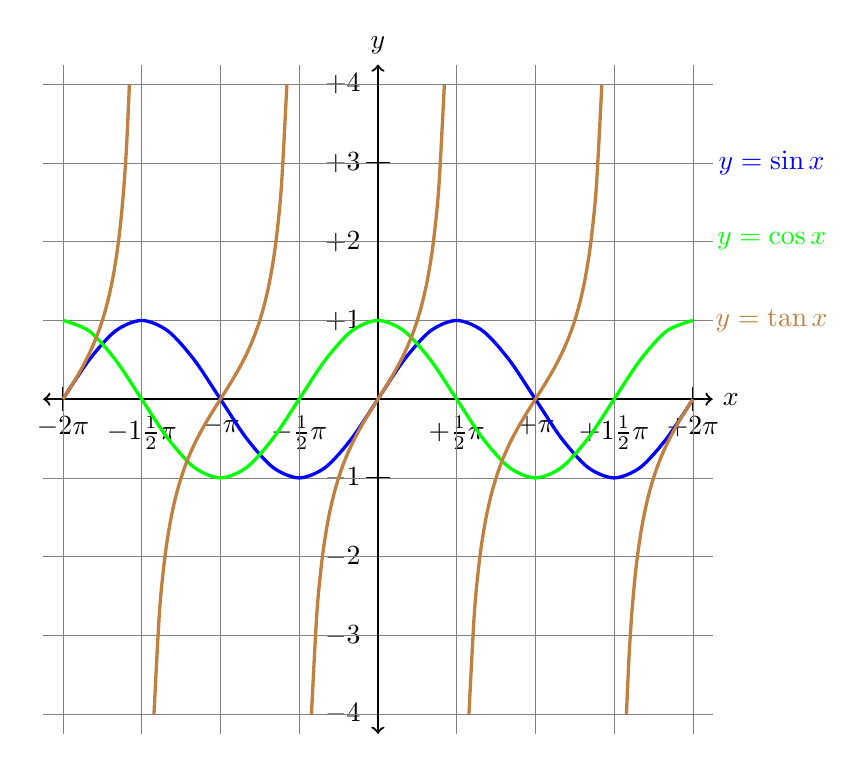
\begin{tikzpicture}[help lines/.style={black!50,very thin}]
	\foreach \x / \r in {-4/-2\pi,-3/-1\frac{1}{2}\pi,-2/-\pi,-1/-\frac{1}{2}\pi,+1/+\frac{1}{2}\pi,+2/+\pi,+3/+1\frac{1}{2}\pi,+4/+2\pi} \draw (\x,-0.15) -- (\x,+0.15) node[below=7] {$\r$};
	\foreach \y in {-4,-3,-2,-1,+1,+2,+3,+4} \draw (-0.15,\y) -- (+0.15,\y) node[left=7] {$\y$};
	\draw[help lines] (-4.25,-4.25) grid (4.25,4.25);
	\draw[<->,thick] (-4.25,0)--(4.25,0) node[right] {$x$};
	\draw[<->,thick] (0,-4.25)--(0,4.25) node[above] {$y$};
	\draw[very thick,color=blue ] plot [domain={(-2*pi)*(2/pi))}:{(+2*pi)*(2/pi)},smooth] (\x,{sin(\x*pi/2 r)});
	\draw[very thick,color=green] plot [domain={(-2*pi)*(2/pi))}:{(+2*pi)*(2/pi)},smooth] (\x,{cos(\x*pi/2 r)});
	\foreach \i in {0,...,4} \draw[very thick,color=brown] plot [domain={((\i-2)*pi-rad(atan(4))*ceil(\i/4))*(2/pi)}:{((\i-2)*pi+rad(atan(4))*ceil((4-\i)/4))*(2/pi)},smooth] (\x,{tan(\x*pi/2 r)});
	\node[blue ] at (5,3) {$y = \sin x$};
	\node[green] at (5,2) {$y = \cos x$};
	\node[brown] at (5,1) {$y = \tan x$};
\end{tikzpicture}

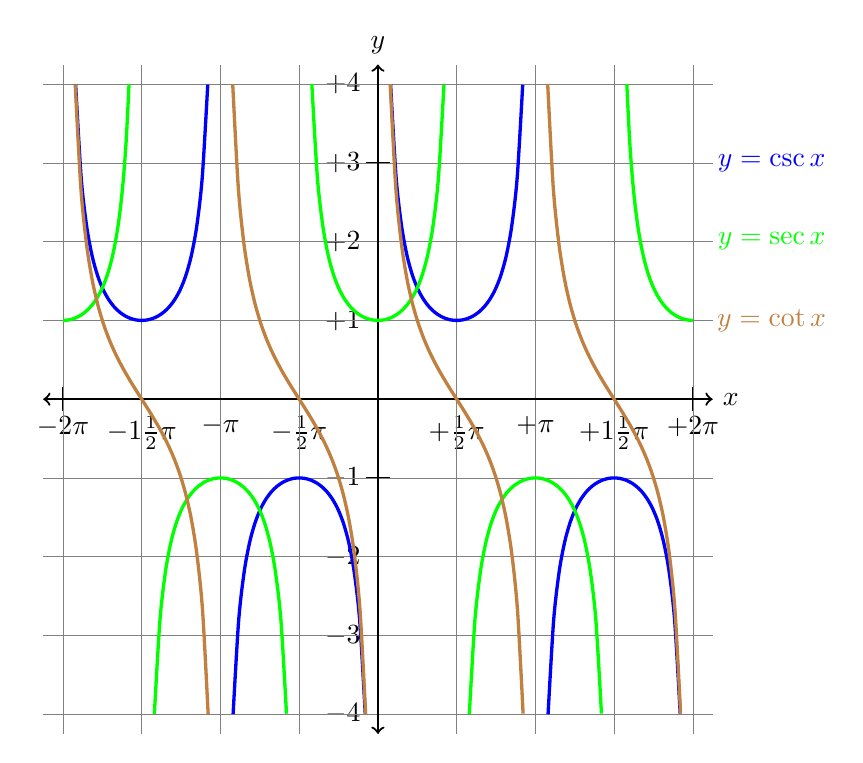
\begin{tikzpicture}[help lines/.style={black!50,very thin}]
	\foreach \x / \r in {-4/-2\pi,-3/-1\frac{1}{2}\pi,-2/-\pi,-1/-\frac{1}{2}\pi,+1/+\frac{1}{2}\pi,+2/+\pi,+3/+1\frac{1}{2}\pi,+4/+2\pi} \draw (\x,-0.15) -- (\x,+0.15) node[below=7] {$\r$};
	\foreach \y in {-4,-3,-2,-1,+1,+2,+3,+4} \draw (-0.15,\y) -- (+0.15,\y) node[left=7] {$\y$};
	\draw[help lines] (-4.25,-4.25) grid (4.25,4.25);
	\draw[<->,thick] (-4.25,0)--(4.25,0) node[right] {$x$};
	\draw[<->,thick] (0,-4.25)--(0,4.25) node[above] {$y$};
	\foreach \i in {0,...,3} \draw[very thick,color=blue ] plot [domain={((\i-2)*pi+rad(asin(1/4)))*(2/pi)}:{((\i-1)*pi-rad(asin(1/4)))*(2/pi)},smooth] (\x,{cosec(\x*pi/2 r)});
	\foreach \i in {0,...,4} \draw[very thick,color=green] plot [domain={((\i-2)*pi-rad(acos(1/4))*ceil(\i/4))*(2/pi)}:{((\i-2)*pi+rad(acos(1/4))*ceil((4-\i)/4))*(2/pi)},smooth] (\x,{sec(\x*pi/2 r)});
	\foreach \i in {0,...,3} \draw[very thick,color=brown] plot [domain={((\i-2)*pi+rad(atan(1/4)))*(2/pi)}:{((\i-1)*pi-rad(atan(1/4)))*(2/pi)},smooth] (\x,{cot(\x*pi/2 r)});
	\node[blue ] at (5,3) {$y = \csc x$};
	\node[green] at (5,2) {$y = \sec x$};
	\node[brown] at (5,1) {$y = \cot x$};
\end{tikzpicture}

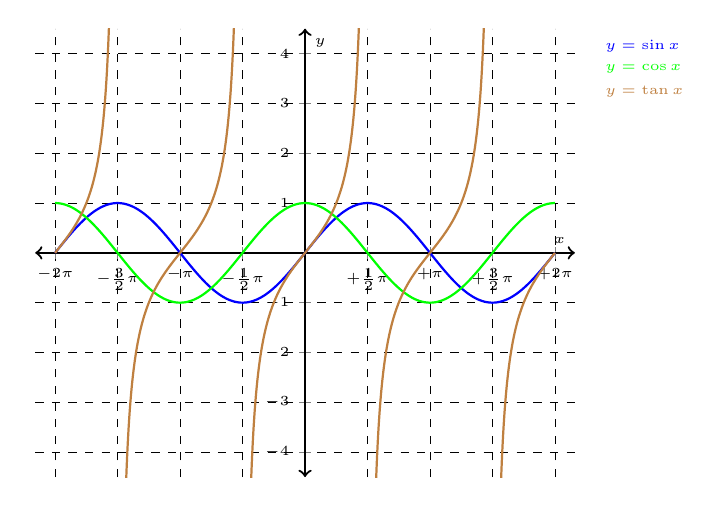
\begin{tikzpicture}
	\begin{axis}[
			axis lines=middle,
			axis line style={thick,<->},
			xmin=-2*pi-0.5,xmax=2*pi+0.5,ymin=-4.5,ymax=4.5,
			ytick={-4,-3,-2,-1,1,2,3,4},
			xtick={-2*pi,-1.5*pi,-pi,-0.5*pi,0,0.5*pi,pi,1.5*pi,2*pi},
			xticklabels={$-2\pi$,$-\frac{3}{2}\pi$,$-\pi$,$-\frac{1}{2}\pi$,$0$,$+\frac{1}{2}\pi$,$+\pi$,$+\frac{3}{2}\pi$,$+2\pi$},
			tick label style={font=\tiny},
			grid=major,
			major grid style={dashed,very thin,black},
			every axis plot post/.append style={thick},
			label style={font=\tiny},
			xlabel=$x$,
			ylabel=$y$,
			smooth,
			%clip=false,restrict y to domain=-4:4,
			legend style={
					font=\tiny,
					legend cell align=left,
					legend pos=outer north east,
					draw=none,
					empty legend},
			legend entries={[blue]$y=\sin x$,[green]$y=\cos x$,[brown]$y=\tan x$}
			]
	\addplot[domain=-2*pi:2*pi,samples=200,blue]{sin(deg(x))};
	\addplot[domain=-2*pi:2*pi,samples=200,green]{cos(deg(x))};
	%\addplot[domain=-2*pi:2*pi,samples=200,brown]{tan(deg(x))};
	\addplot[domain=-2  *pi:-1.5*pi,samples=200,brown]{tan(deg(x))};
	\addplot[domain=-1.5*pi:-0.5*pi,samples=200,brown]{tan(deg(x))};
	\addplot[domain=-0.5*pi: 0.5*pi,samples=200,brown]{tan(deg(x))};
	\addplot[domain= 0.5*pi: 1.5*pi,samples=200,brown]{tan(deg(x))};
	\addplot[domain= 1.5*pi: 2  *pi,samples=200,brown]{tan(deg(x))};
	\end{axis}
\end{tikzpicture}
	

\end{document}
